
\documentclass[10pt, journal, compsoc, a4paper]{IEEEtran}

\usepackage[pdftex]{graphicx}
\usepackage{listings}
\usepackage{todonotes}

% correct bad hyphenation here
\hyphenation{op-tical net-works semi-conduc-tor}


\begin{document}
\title{Extending Mocapy++ with a mixed probability distribution\\Advanced Topics In Data Modeling}

\author{\IEEEauthorblockN{Kasper Nybo Hansen}
\IEEEauthorblockA{Dept. of Computer Science\\
University of Copenhagen\\
Copenhagen, Denmark\\
nybo@diku.dk}
}

% make the title area
\maketitle

\begin{abstract}
Mocapy++ is a C++ toolkit for learning and inference in dynamic Bayesian networks. This report describes the implementation, testing and results of extending Mocapy++ with a new node. 

The new node is a mixed node, allowing both discrete and continuous values. The continuous part of the node is a gaussian distribution. The new node is used to calculate a probabilistic model of hydrogen bonding in protein structures. The probabilistic model is learned from a provided dataset.
\end{abstract}

\begin{IEEEkeywords}
Mocapy++; DIKU; Dynamic Bayesian networks; Mixed probability distribution
\end{IEEEkeywords}


\section{Introduction} % (fold)
\label{sec:introduction}

This section gives a short introduction to the theory of inference and learning in Bayesian networks that are relevant to the implementation that are presented later in the paper.

\subsection{Dynamic Bayesian Network} % (fold)
\label{sub:dynamic_bayesian_network}
A Bayesian network consists of a Directed Acyclic Graph where the nodes are random variables. Each edge in a Bayesian network represents a probabilistic dependency. Figure \ref{fig2} shows a Bayesian network where e.g. the probability of observing $o1$ is dependent on $h1$. We call the node $o1$ the observed node and $h1$ and $h2$ the hidden nodes. 

\begin{figure}[ht]
\centering
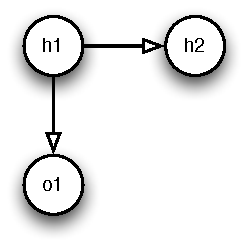
\includegraphics[width=0.2\textwidth]{figures/fig2.pdf}
\caption{Example of a bayesian network, $o_1$ is the observed node and $h_1$ and $h_2$ are hidden nodes}
\label{fig2}
\end{figure}

We can learn the the probabilities of the hidden node, through the observed node, and this process is called inference. Mocapy++ used Gibbs sampling to do inference on the hidden nodes. 

In this paper the observed node is a new node type called a mixed node. This node can only have one parent, and this parent and the parent needs to return discrete values. The number of different values the parent node can take, is also called the parent nodes size. The size of the parent node to a mixed node can be arbitrarily large i.e. the value can take integer values in the range $[0,n]$.

When doing inference we learn the parameters of the hidden nodes based on the observations made in the mixed node. The goal is to learn the distribution of the values of the parent mode. 

The parameter learning is done through the Expectation Maximization (EM) algorithm. In the E-step the values of the hidden nodes are inferred using the parameter settings present at that current time. To approximate the probability distributions of the hidden nodes, Mocapy++ uses Gibbs sampling.

In the M-step the inferred values of the hidden nodes are used to update the parameters of the DBN. These two steps are repeated until convergence is reached, or some maximum number of cycles has been run. 

% subsection dynamic_bayesian_network (end)

\subsection{Mixed distribution} % (fold)
\label{sub:mixed_distribution}
The mixed node has a mixed distribution.

The mixed distribution can be divided into two parts. A discrete and continuous part. Let $X$ be a random variable that takes values in the set $S$. We then define the discrete part as the countable set $D \subseteq S$, and the continuous part as $C \subseteq S$. We define a mixed distribution as a distribution that has the following two properties

\begin{center}
  \begin{itemize}
    \item $0 < P(x \in D) < 1$
    \item $P(x \in C) = 0$
  \end{itemize}   
\end{center}
the first property ensures that no element in the discrete set $D$ has zero probability. The second property ensures that $C$ is a continuous set, thus there are infinite many elements, and the probability of drawing a single element is thus $0$. 

The discrete part of the distribution can be described by a distribution table. The distribution table in the mixed node consist of two entries that sums to exactly $1$. This table is called the conditional probability density (CPD). The first entry describes the probability of the node being a discrete node, the second entry describes the probability of the node being a continuous node. Define $P(X = discrete)$ as the probability that the node is discrete, and $P(X = continuous) = 1-P(X = discrete)$ as the probability that the node is continuous. 

The continuous part of the mixed distribution consist of the Gaussian distribution aka. the normal distribution. The Gaussian is defined as

\begin{equation}
f(x;\mu,\sigma) = \frac{1}{\sqrt{2\pi\sigma^2}} e^{ -\frac{(x-\mu)^2}{2\sigma^2} }  
\end{equation}
where $\mu$ is the mean value, and $\sigma$ is the standard deviation.

We wish to estimate the parameters of the discrete and continuous distribution. We can do this by the maximum likelihood method. For the discrete case, the maximum likelihood can be calculated as

\begin{equation}
  \hat{P}(X = discrete) = \frac{\#discrete}{\#total}
  \label{eq3} 
\end{equation}
and by definition we have that the maximum likelihood of encountering a continuous node is
\begin{equation}
  \hat{P}(X = continuous) = 1 - \hat{P}(X = discrete)
\end{equation}
where $\#discrete$ denotes the number of discrete observation and $\#total$ denotes the total number of observations.


When estimating the Gaussian variables $\mu$ and $\sigma$ we use the maximum likelihood function for the Gaussian, i.e.
\begin{equation}
  \ln(\mu, \sigma^2) = -\frac{n}{2}\ln(2\pi) - \frac{n}{2}\ln\sigma^2 - \frac{1}{2\sigma^2}\sum_{i=1}^n (x_i-\mu)^2.
\end{equation}
we wish to maximize this function, so we take the derivative and find the stationary points. Doing this yields
\begin{equation}
  \hat{\mu} = \overline{x} \equiv \frac{1}{n}\sum_{i=1}^n x_i, \qquad \hat{\sigma}^2 = \frac{1}{n} \sum_{i=1}^n (x_i - \overline{x})^2
  \label{eq1}
\end{equation}
so the parameters of the Gaussian distribution can be estimated from the continuous samples by the two equations in \ref{eq1}. 


Having the parameters of the distribution models in the mixed model we would also like to be able to calculate the likelihood of a sample belonging to the mixed node. We can calculate this likelihood in the following way. Let the sample consist of two elements $s = {d, e}$. The likelihood of $s$ can then be calculated as
\begin{equation} 
L(s) = 
\left\{
\begin{array}{ll} 
  \hat{P}(discrete) & \mathbf{if } d = 0  \\
  \hat{P}(continuous) \frac{1}{\sqrt{2\pi\hat{\sigma}^2}} e^{ -\frac{(e-\hat{\mu})^2}{2\hat{\sigma}^2} }  & \mathbf{if } d = 1    
  \label{eq6}
\end{array} 
\right. 
\end{equation} 
where $\hat{P}(discrete)$ denotes the estimated probability of observing a discrete node, and likewise $\hat{P}(continuous)$. We multiply the Gaussian with $\hat{P}(continuous)$ in order to normalize the mixed distribution.
% subsection mixed_distribution (end)

% subsection d (end)

\subsection{Applications to Hydrogen bounding} % (fold)
\label{sub:applications_to_hydrogen_bounding}
The mixed distribution applies to hydrogen bonding in the following way. A hydrogen bound has two states:

\begin{itemize}
  \item A bond is present or it is not present
  \item If the bond is present it has an energy associated
\end{itemize}

Under the assumption that the energy of a hydrogen bonding can be modeled by a Gaussian probability distribution we can model a hydrogen bond in the following way. The discrete distribution is modeling the first boolean case, i.e. "Is the bond present or not?". If the bond is present, the Continuous part can be used to to find the energy, $E$, of the bond.

The assumption that the energy is modeled by a Gaussian distribution is somewhat crude. Although simple investigation of the energies present in the supplied dataset, actually indicates that the energy could be modeled by a Gaussian distribution. 
% subsection applications_to_hydrogen_bounding (end)


% section introduction (end)

\section{Implementation} % (fold)
\label{sec:implementation}
The following section describes in detail the implemented mixed node.

\subsection{Adding the mixed node} % (fold)
\label{sub:adding_the_mixed_node}
The mixed node is added to the framework by creating a new node type in \texttt{dbn.h}. The new type defines the name of the density and ESS classes, furthermore it defines the typename, which is called \texttt{mixednode}. A new node type is also added to \texttt{node.h}, called \texttt{mixed}.

In order to create new nodes, the \texttt{nodefactory} class is extended with a new method called \texttt{new\_mixed\_node}. The new mixed node takes the following parameters

\begin{itemize}
  \item Size: this is only allowed to be 2, but is present for the sake of future works
  \item Name: used in text output, Optional
  \item Init\_random: Randomly initialize the CPD, Optional
  \item CPD: User specified CPD, Optional
  \item Means: User specified Gaussian means array, Optional
  \item Variance: User specified variance array, Optional
\end{itemize}

In this report we assume that the node size of our mixed node is always $2$, this assumption also has the effect that the Gaussian is one dimensional. I have included the node size as an argument, in order to make it easy to expand the mixed node in future works, so it can handle multidimensional Gaussian distributions. 

There are several optional arguments to the \texttt{new\_mixed\_node} method. If nothing is specified in the optional arguments, the following default behavior is applied. If nothing is specified in init\_random the node will be initialized with a uniform CPD. If nothing is specified in the means and variance arguments then these are initialized randomly.

The node consist of four files: \texttt{mixedess.h}, \texttt{mixedess.cpp}, \texttt{mixeddensities.h} and \texttt{mixeddensities.cpp}. All four files resides in the \texttt{mixed} directory of the \texttt{src} folder.

The following sub-sections elaborate on the individual parts of the mixed node implementation.

% subsection adding_the_mixed_node (end)

\subsection{ESS - inference} % (fold)
\label{sub:ess}
There are two main steps in the framework. The first step is the \emph{E-step}. The E-step is the inference step, where the values of the hidden nodes are inferred by using the set of samples generated by the sampler. The sampler used in this project is the Gibbs sampler that comes with Mocapy++.

Each time a node is sampled the \textbf{E}xpected \textbf{S}ufficient \textbf{S}tatistics (ESS) class is updated. The ESS class acts as a container where the data neccessary to calculate the nodes parameters are stored. For the mixed node, this means storing the following data:

\begin{itemize}
  \item Number of discrete and continuous observations
  \item The energy stored in a way so the Gaussian model parameters can be calculated
\end{itemize}
the parameters needs to be stored for each value that the parent node can take. I.e the size of the tables stored in the ESS, depends on the size of the parent node.

I have implemented the ESS class in the file \texttt{mixed/mixedess.cpp}. The class is responsible for collection data about the sample points, so they can be used later in the density class. Both tables are stored in the ESS array.

The \texttt{mixedess} class stores two tables for later retrieval in the density class. 

Both tables are populated in the class method \texttt{add\_ptv}. This method takes a vector as input. The vector has the format
\begin{equation}
  \{Parent\ value, Indicator, Energy\}
\end{equation}
and is called \texttt{ptv}.


If $Indicator=0$ then we know that the sample is a discrete sample, otherwise it must be a continuous sample.

The first table stores the number of observations of discrete and continuous nodes. It has size equal to the parent size $\times$ node size. The table has a row for each value the parent can take. For each value of the parent the ESS thus stores the number of discrete and the number of continuous nodes. Define the parent with value $i$ as $p_i$, and define the size of the parent node as $n$. Then the following table yields an outline of the first table stored in the ESS
\begin{center}
  \begin{tabular}{c | c | c}
  $p_0$ & \#Discrete for $p_0$ & \#Continuous for $p_0$ \\
  $p_1$ & \#Discrete for $p_1$ & \#Continuous for $p_1$ \\
  \vdots & \vdots & \vdots \\
  $p_{n-1}$ & \#Discrete for $p_{n-1}$ & \#Continuous for $p_{n-1}$ 
  \end{tabular}  
\end{center}
where the entries is the number of discrete and continuous observations for a particular parent.

The second table stored in the ESS has the size parent size $\times$ node size. For each parent value we store two entities. The first entity is the sum of the energies, and the second is the sum of the squared energies. Define all the energy samples belonging to parent $p_i$ as $E_i$, then for each continuous sample with parent value $p_i$ we sum the energy in one column and the sum the energy squared in the other column. An outline of the table can be seen in the following table
\begin{center}
  \begin{tabular}{c | c | c}
  $p_0$ & $\sum_{\forall e \in E_0} e$ & $\sum_{\forall e \in E_0} e^2$ \\
  $p_0$ & $\sum_{\forall e \in E_1} e$ & $\sum_{\forall e \in E_1} e^2$ \\
  \vdots & \vdots & \vdots \\
  $p_{n-1}$ & $\sum_{\forall e \in E_{n-1}} e$ & $\sum_{\forall e \in E_{n-1}} e^2$ \\
  \end{tabular}  
\end{center}         

Note throughout this report, when otherwise not noted, the first column (The column containing the parent value) is not present in the implemented arrays, since this is stored implicit in the array data structure and can be accessed by indexing. It is solely shown in the outline tables for clarity. 

%subsection ess (end)

\subsection{Densities - parameter estimation} % (fold)
\label{sub:densities}
The second step of the framework is the \emph{M-step}. In the M-step we update the parameters of the model, e.g. updating the CPD.

The density class is implemented in the file \texttt{mixed/mixeddensities.cpp}. 

Parameter estimation is done in the method \texttt{estimate}. The function takes the ess array from the ESS class as argument, and calculates the CPD, means and variance arrays. The CPD is calculated directly from the array containing the number of discrete and the number of continuous observations. The CPD is thus an array where each row contains the probability of observing a continuous and discrete node, given a parent value represented by the row index. 

The estimated probability of observing a discrete value, $\hat{P}(Discrete)$, is calculated as shown in (\ref{eq3}) 

The outline of the CPD table can be seen in the following table 

\begin{center}
  \begin{tabular}{c | c | c}
  $p_0$ & $\hat{P}(Discrete)$ & $\hat{P}(Continuous)$\\
  $p_1$ & $\hat{P}(Discrete)$ & $\hat{P}(Continuous)$\\
  \vdots & \vdots & \vdots \\
  $p_{n-1}$ & $\hat{P}(Discrete)$ & $\hat{P}(Continuous)$ 
  \end{tabular}  
\end{center}

We can calculate the estimated mean and variance of the Gaussian in the following way. Remember we stored the sum of the energies and the sum of the squared energies in the ess array in the ESS class. Furthermore we stored the number of discrete and continuous observations. In both cases we stored the numbers for each parent value. We can thus calculate the mean for the parent value $i$ as
\begin{equation}
  \hat{\mu}_i = \frac{sum_i}{total_i} 
\end{equation}
where $sum_i$ is the total sum of the energies for the parent value $i$, and $total_i$ is the total number of continuous observations for the parent value $i$. The result is a table with the following structure
\begin{center}
  \begin{tabular}{c | c }
  $p_0$ & $\hat{\mu}_1$ \\
  $p_1$ & $\hat{\mu}_2$ \\
  \vdots & \vdots \\
  $p_{n-1}$ & $\hat{\mu}_{n-1}$  
  \end{tabular}  
\end{center}


The variance can be calculated as shown in (\ref{eq1}). From the ess array we also have the squared sum of the energies. The variance is then calculated as
\begin{equation}
  \hat{\sigma_i}^2 = \frac{sumsquared_i}{total_i} - \hat{\mu_i}^2
\end{equation}

where $sumsquared_i$ is the sum of the squared values cumming from the ess. The resulting variance table looks like
\begin{center}
  \begin{tabular}{c | c }
  $p_0$ & $\hat{\sigma_1}^2$ \\
  $p_1$ & $\hat{\sigma_2}^2$ \\
  \vdots & \vdots \\
  $p_{n-1}$ & $\hat{\sigma_{n-1}}^2$  
  \end{tabular}  
\end{center}


\subsection{Densities - likelihood} % (fold)
\label{sub:densities_likelihood}
The likelihood calculation is done in the method \texttt{get\_lik}. The method takes two variables and returns a \texttt{double}. The first variable is the \texttt{ptv} and the second variable is a \texttt{boolean} value indicating if the result should be logarithmic scaled.

Recall that the \texttt{ptv} is a 3-tuple consisting of the values $\{Parent\ value, Indicator, Energy\}$. As usual we define the parent value as $p_i$. Given the \texttt{ptv}, we wish to answer the question, `How likely is it to see this sample given the current model configuration?'. 

We can answer this question in the following way.  If the indicator is $0$ we return the likelihood of seeing a discrete value. This value can be found by making a lookup in the CPD under the given parent value. 

If the indicator is $1$, we know we are in the continuous case. We thus calculate the likelihood as (\ref{eq6}), i.e.

\begin{equation}
  \hat{P}(continuous) \frac{1}{\sqrt{2\pi\hat{\sigma_i}^2}} e^{ -\frac{(e-\hat{\mu_i})^2}{2\hat{\sigma_i}^2} }
  \label{eq20}
\end{equation}
where $\hat{P}(continuous)$ can be found by making a lookup in the CPD table, and where $\mu_i$ and $\sigma_i$ can be found in the means and variances table by making a lookup under $p_i$.


Due to limited precision, the likelihood can become $0$. This can happen when (\ref{eq20}) is close to $0$. If this happens and the method is called with the boolean flag set to true, an error will occur because we cannot take the logarithm of 0. To remove this problem, we test if the likelihood is calculated as zero. If it is, we set it to the constant \texttt{\_MIN\_TRANSITION}. This ensures that we always will take the logarithm of a positive number.

% subsection densities_likelihood (end)


\subsection{Densitites - sampling} % (fold)
\label{sub:densitites_sampling}
The sampling is done in the method \texttt{sample}. The method takes one argument, namely a parent value. and returns a tuple of two elements. 

The sampling is done in the following way. A random number $r$ is generated such that $0 < r < 1$. 

A lookup in the CPD for the given parent value is performed, yielding the probability of observing a discrete node. Call this probability the \emph{threshold}. If $r \leq threshold$ then the return value of the \texttt{sample} method is the tuple $<0,0>$. The first element in the tuple is the indicator value, and the second is the energy. This energy is assumed to be zero when discrete values are observed.

If $r > threshold$ then we need to sample from the Gaussian distribution. In order to sample from the Gaussian distribution we use the method \texttt{normal\_multivariate} found in \texttt{utils/random\_data.cpp}. This function requires 5 arguments. The first being the dimension of the Gaussian, the second being the number of samples, the third is the standard deviation, the fourth is the mean and the fifth is the random generator to be used. 

We set the dimension and the number of samples to $1$. From the estimate function we have the means and the variances of each of the parent values. We can thus make a lookup in these arrays and find the mean and variance. In order to calculate the standard deviation we take the square root of the variance. The return value of \texttt{normal\_multivariate} is a vector of samples. In our case we only asked for one sample, so the vector has a length of $1$. Call the generated sample for $s$. We then make the \texttt{sample} function return the tuple $<1, s>$.

% subsection densitites_sampling (end)


% subsection densities (end)
%section implementation (end)

\section{Testing of implementation} % (fold)
\label{sec:testing_of_implementation}

This section describes the testing done to ensure that the implemented mixed node works as supposed. 2 tests are performed.

\subsection{Test of inference and sampling} % (fold)
\label{sub:test_of_sampling}
In this test we would like to confirm that the samples drawn from the mixed node corresponds to the nodes parameters. The test is done with a hidden node size of $1$.

The test in \texttt{examples/hmm\_mixed2.cpp} creates two DBN's. The first network is initialized with randomly picked CPD, mean and variance. After initialization, multiple samples is drawn from the network. These samples is then used to train a second network. 

We expect the two networks to have almost identical parameters, i.e. we expect the second network to be able to learn the parameters of the first network that generated the sample points.

The result of the test is

\begin{verbatim}
to0:
  Node: Mixed, size: 1 2 
  Mixed CPD: 
  [0.476073 0.523927 ]

  Gaussian means: 
  0.476903 
  Gaussian variances: 
  0.20354 
    
mo0:
  Node: Mixed, size: 1 2 
  Mixed CPD: 
  [0.47202 0.52798 ]

  Gaussian means: 
  0.476937 
  Gaussian variances: 
  0.203367 
\end{verbatim}
As we can see the two nodes are almost identical, which confirms that the inference is working as supposed.

In order to test the samples drawn from the discrete part, the sampled data is exported, and the indicator values is isolated. From these values a histogram is made. the expectation is that the distribution of the sampled indicator values, is close to the randomly picked CPD. The CPD in this case is $[0.476073, 0.523927]$. Figure \ref{fig3} shows the histogram of the indicator values.

\begin{figure}[ht]
\centering
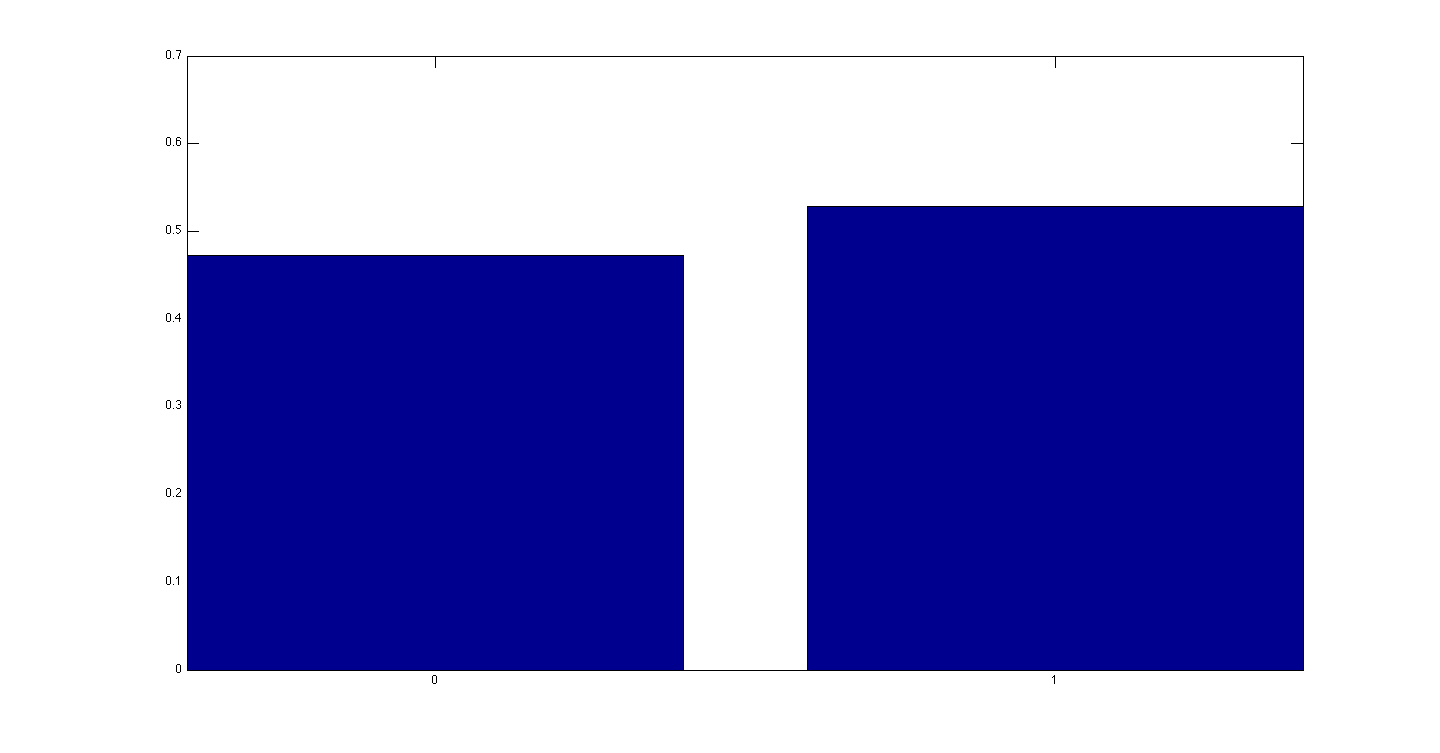
\includegraphics[width=0.5\textwidth]{figures/fig3.png}                                                                             
\caption{Histogram of the indicator values. The distribution of the two, should resemble the randomly generated PCD. The distribution of the drawn indicator values is $[0.47202,  0.52798]$, compared to the randomly picked CPD: $[0.476073, 0.523927]$. There are some discrepancies, but still acceptable.}
\label{fig3}
\end{figure}

In order to show that the sampling of the continuous case is correct, we have extracted the data points generated by the first DBN. The data points consist of both discrete and continuous samples. By isolating the continuous samples, and making a histogram, we expect the histogram to resemble a Gaussian distribution, i.e. take the shape of the bell curve. 

The histogram can be seen on figure \ref{fig1}. On top of the histogram, we have plotted a Gaussian probability density function with the mean and variance equal to the model parameters, i.e. $\hat{\mu} = 0.4769$ and $\sigma^2 = 0.20354$. As can be seen from figure \ref{fig1} the histogram approximates the Gaussian very well, and the conclusion must be that the samples drawn from the continuous part of the distribution is correct.

\begin{figure}
\centering
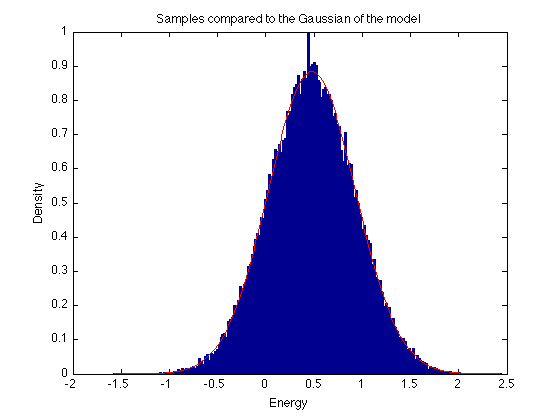
\includegraphics[width=0.5\textwidth]{figures/fig1.png}
\caption{Histogram of the samples drawn from the Gaussian part of the mixed distribution. Red curve is a Gaussian probability distribution with the parameters randomly drawn, i.e. $\hat{\mu} = 0.4769$ and $\sigma^2 = 0.20354$. Note that the distribution is not normalized!}
\label{fig1}
\end{figure}

%subsection test_of_sampling (end)



\subsection{Test of save and load} % (fold)
\label{sub:test_of_save_and_load}
The saving function of the mixed node is tested in the following way. 

The previous test, \texttt{hmm\_mixed2.cpp}, saves intermediate model states in a file called \texttt{mixed\_hmm2.dbn}. We expect to be able to load this file, and thereby recreating the model. The class responsible for loading the file and recreating the model is the \texttt{dbn} class. 

In \texttt{hmm\_mixed3.cpp} a test case is created that loads the file \texttt{mixed\_hmm2.dbn} generated by hmm\_mixed2, recreates the model and prints it to the screen. We expect the loaded model to be identical to the final model calculated in the \texttt{hmm\_mixed2.cpp} which is also shown above.

The output of \texttt{hmm\_mixed3.cpp} is 

\begin{verbatim}
*** LOADED MODEL WITH PARAMETERS ***
h1: mh0
  Node: Discrete, size: 1 
  1 

o1: mo0
  Node: Mixed, size: 1 2 
  Mixed CPD: 
  [0.47202 0.52798 ]

Gaussian means: 
  0.476937 
Gaussian variances: 
  0.203367   
\end{verbatim}
which is identical to the output in the pervious test. We can therefore conclude that the saving, and loading of the model works as supposed.
% subsection test_of_save_and_load (end)


% section testing_of_implementation (end)


\section{Results on supplied dataset} % (fold)
\label{sec:results}
A network with the mixed node has been setup, and the network has been trained on the two provided datasets. Several different parent sizes have been tested. A parent size of $1$, yields only one Gaussian distribution which doesn't fit the training data very well. A parent size of $5$ seems to cause overfitting, and some of the $5$ Gaussians have a strong overlap. A parent size of $2$ is found to yield the best results. Both test cases in the section is run with parent size $2$. The test is run with a burn in value of $10$. The network keeps running until convergence is reached. Convergence is reached when there is no improvement in the log-likelihood 30 times in a row.

Both test can be found in the file \texttt{examples/hmm\_mixed6.cpp}. The following two subsections elaborate on the results found.

\subsection{Energy\_CO dataset} % (fold)
\label{sub:energy_co_dataset}

The result of running the implementation with the \texttt{energy\_CO} data set as input and a hidden node size equal to $2$ can be seen in the following output.

\begin{verbatim}
LL= -1.38917580670968
h1: h1
  Node: Discrete, size: 2 
  0.89847 0.10153 


o1: o1
  Node: Mixed, size: 2 2 
  Mixed CPD: 
  [0.60764 0.39236 ]
  [2.1166e-05 0.99998 ]

  Gaussian means: 
  -1.6738 -2.4113 
  Gaussian variances: 
  0.88943 0.22712 


h2: h2
  Node: Discrete, size: 2 2 
  [0.89229 0.10771 ]
  [0.20366 0.79634 ]
\end{verbatim}

Figure \ref{fig4} illustrates the output, where the \texttt{energy\_CO} data set is plotted as a histogram, where the two gaussians produced by the DBN is superimposed onto. 

\begin{figure}[ht]
\centering
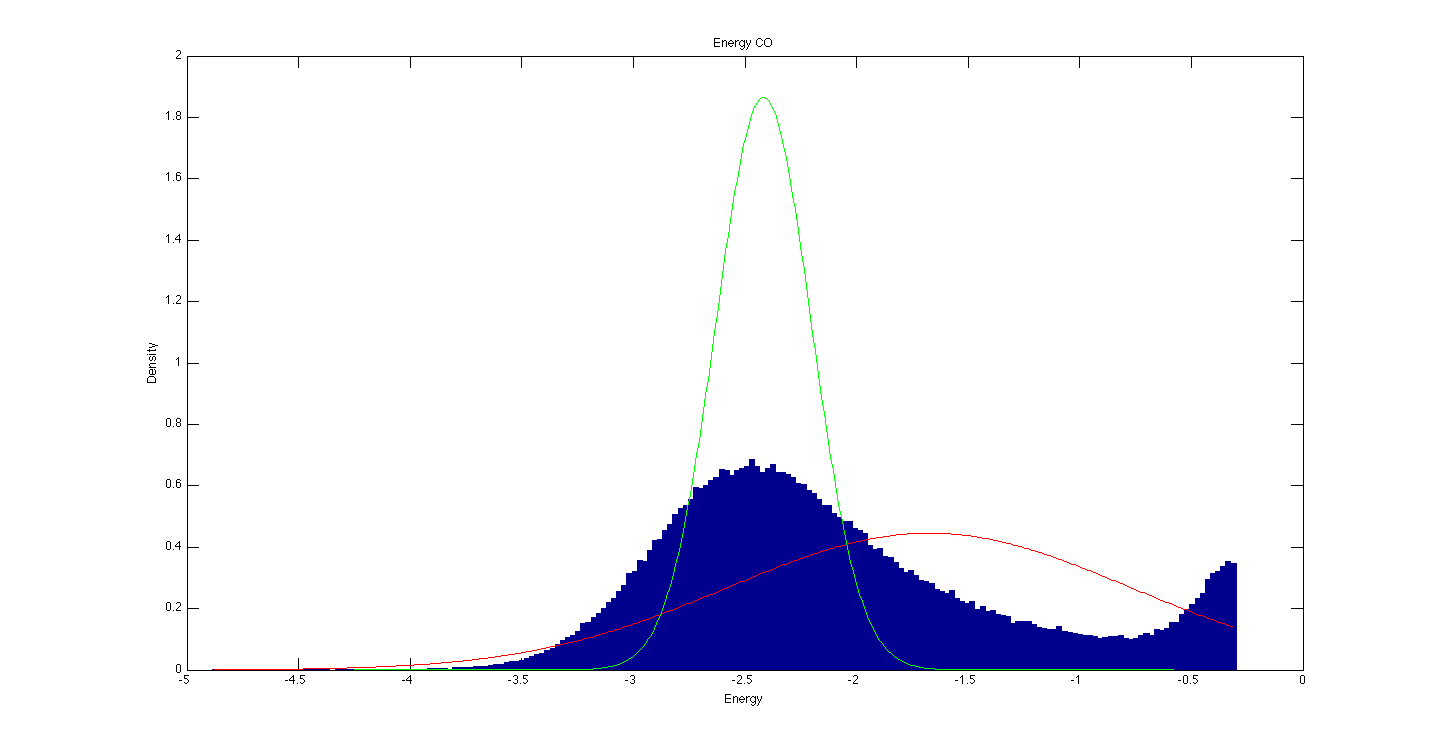
\includegraphics[width=0.5\textwidth]{figures/fig4.png}
\caption{The continuous samples from the energy\_CO dataset plotted as a histogram. The red and green lines are the 2 Gaussians found by the DBN.}
\label{fig4}
\end{figure}


% subsection energy_co_dataset (end)

\subsection{Energy\_NH dataset} % (fold)
\label{sub:energy_nh_dataset}
The result of running the implementation on the \texttt{energy\_NH} dataset yields the following output

\begin{verbatim}
LL= -1.58744875772879
h1: h1
  Node: Discrete, size: 2 
  0.99643 0.0035714 

o1: o1
  Node: Mixed, size: 2 2 
  Mixed CPD: 
  [0.76625 0.23375 ]
  [0.081073 0.91893 ]

Gaussian means: 
  -0.97857 -2.1716 
  Gaussian variances: 
  0.47761 0.54614 

h2: h2
  Node: Discrete, size: 2 2 
  [0.70649 0.29351 ]
  [0.15369 0.84631 ]
\end{verbatim}

A histogram of the continuous part of the dataset can be seen on figure \ref{fig5} along with two superimposed Gaussians that have the estimated $\mu$ and $\sigma^2$ from the DBN.

\begin{figure}[ht]
\centering
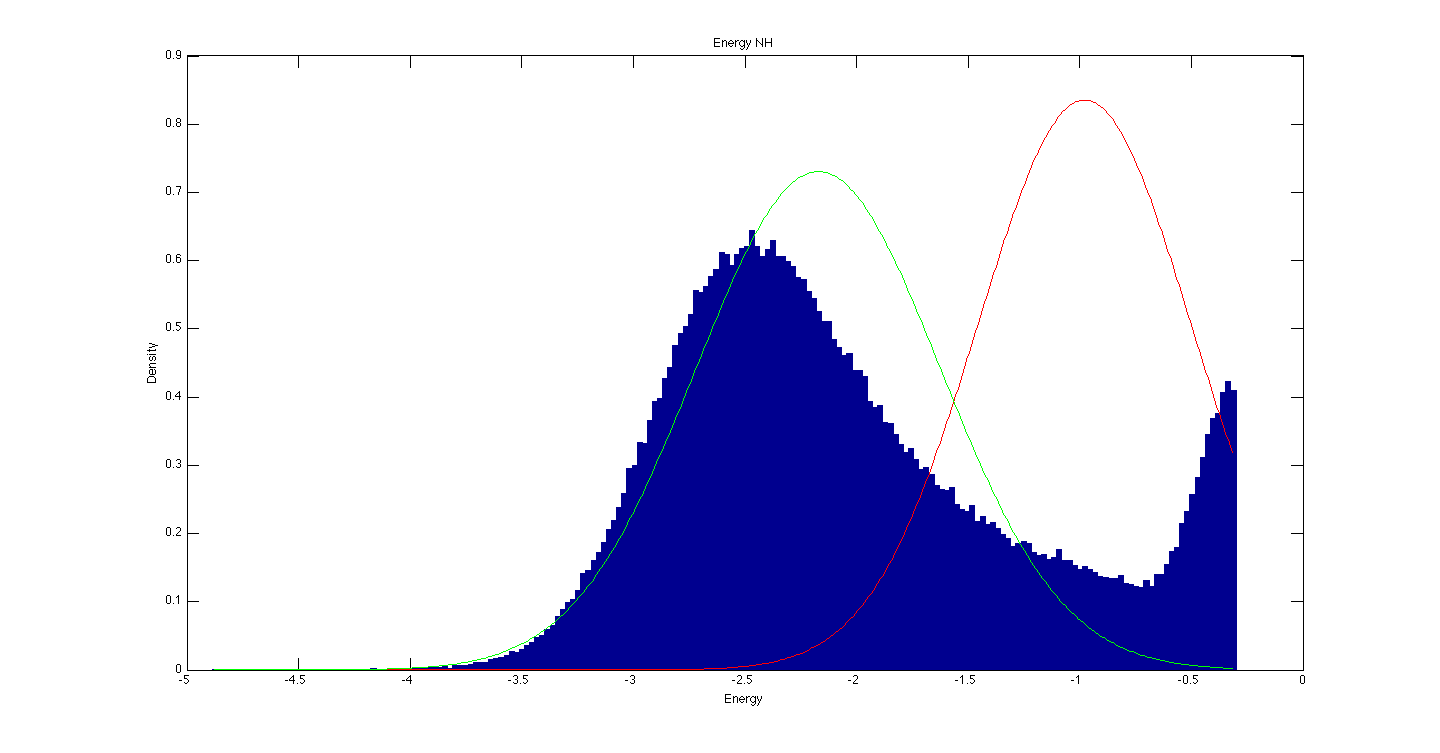
\includegraphics[width=0.5\textwidth]{figures/fig5.png}
\caption{The continuous samples from the energy\_NH dataset plotted as a histogram. The red and green lines are the 2 Gaussians found by the DBN.}
\label{fig5}
\end{figure}

% subsection energy_nh_dataset (end)






% section results (end)   

\section{Future work} % (fold)
\label{sec:future_work}
The mixed node presented in this report can only handle one dimensional gaussian nodes. A really neat feature, would be, to be able to use the existing nodes as the continuous node in the mixed node. Future work could involve making the mixed node general, adopting an arbitrarily other node as it's continuous part. This would also remove the duplicate code to calculate the Gaussian likelihood that is present in the presented mixed node. And at the same time add a degree of flexibility to the mixed node.

Another nice feature to have, would be to be able to handle multidimensional Gaussian distributions. This feature would be enabled with the above extension.
% section future_work (end)


\section{Conclusion} % (fold)
\label{sec:conclusion}
The theory behind the mixed distribution has been explained and Mocapy++ has been extending with a mixed node. The node has a discrete and continuous part, where the continuous part consist of a Gaussian distribution. The mixed node is, in it's current state, very stationary, and several suggestions for future work has been presented, especially the possibility to make the mixed node general, giving it the possibility to adopt \emph{any} node as it's continuous part. The node has been used on a supplied dataset consisting of data from hydrogen bondings. The result is that the node performs best with a parent size of $2$. 

% section conclusion (end)


\bibliographystyle{abbrv}
\bibliography{bibliography}
\end{document}